\documentclass[a4paper,12pt]{article}

\usepackage[T2A]{fontenc} 
\usepackage[utf8]{inputenc}
\usepackage[english,russian]{babel}
\usepackage{listings}
\usepackage[dvips]{graphicx}
\usepackage{indentfirst}
\usepackage{color}
\usepackage{hyperref}
\usepackage{amsmath}
\usepackage{amssymb}
\usepackage{geometry}
\geometry{left=1.5cm}
\geometry{right=1.5cm}
\geometry{top=1cm}
\geometry{bottom=2cm}

\graphicspath{{images/}}

\begin{document}
\sloppy

\lstset{
	basicstyle=\small,
	stringstyle=\ttfamily,
	showstringspaces=false,
	columns=fixed,
	breaklines=true,
	numbers=right,
	numberstyle=\tiny
}

\newtheorem{Def}{Определение}[section]
\newtheorem{Th}{Теорема}
\newtheorem{Lem}[Th]{Лемма}
\newenvironment{Proof}
	{\par\noindent{\bf Доказательство.}}
	{\hfill$\scriptstyle\blacksquare$}
\newenvironment{Solution}
	{\par\noindent{\bf Решение.}}
	{\hfill$\scriptstyle\blacksquare$}


\begin{flushright}
	Кринкин М. Ю. группа 504 (SE)
\end{flushright}

\section{Домашнее задание 1}

\paragraph{Задание 1.} Отображение плана выполнения. Физицеский операции. Понятие плана.

В качестве запросов для тестирования выбраны запросы различных классов:
\begin{enumerate}
\item Простой запрос без вложенных запросов

\item Простой запрос с операцией сортировки

\item Запрос с вложенным подзапросом и операцией $IN$

\item Сложный запрос с пятью вложенными подзапросами
\end{enumerate}

\begin{lstlisting}
7.4
   SELECT   PlayerNo, Street + ' ' + HouseNo AS Address
   FROM     Players
   WHERE    Town = 'Stratford';
\end{lstlisting}

\begin{lstlisting}
8.1
   SELECT   PlayerNo, LeagueNo
   FROM     Players
   WHERE    Town = 'Stratford'
   ORDER BY LeagueNo asc;
\end{lstlisting}

\begin{lstlisting}
10.18
   SELECT   PlayerNo, Name
   FROM     Players
   WHERE    PlayerNo IN 
           (
            SELECT   PlayerNo
            FROM     Matches
            WHERE    TeamNo = 1
           );
\end{lstlisting}

\begin{lstlisting}
15.9
   SELECT   PlayerNo
   FROM     Players P
   WHERE    NOT EXISTS 
           (
            SELECT   *
            FROM     Matches M1
            WHERE    PlayerNo = 57
              AND    NOT EXISTS 
                    (
                     SELECT   *
                     FROM     Matches M2
                     WHERE    M1.TeamNo = M2.TeamNo
                       AND    P.PlayerNo = M2.PlayerNo
                    )
           )
     AND    NOT PlayerNo IN 
           (
            SELECT   PlayerNo
            FROM     Matches
            WHERE    TeamNo IN 
                    (
                     SELECT   TeamNo
                     FROM     Teams
                     WHERE    NOT TeamNo IN 
                             (
                              SELECT   TeamNo
                              FROM     Matches
                             )
                    )
           );
\end{lstlisting}

В ходе работы измерялось время генерации плана и время исполнения запроса по мере наполнения базы данных,
при этом в скрипте $UpgradeSportDB4$ была обнаружена ошибка, требуется заменить все комманды типа
\begin{lstlisting}
	INSERT INTO Players VALUES(13070,3170,'12/04/2006',72);
\end{lstlisting}
на запросы вида:
\begin{lstlisting}
	INSERT INTO Penalties VALUES(13070,3170,'12/04/2006',72);
\end{lstlisting}

Сводная таблица результатов:

\begin{tabular}[t]{|c|c|c|c|c|c|}
\hline
\multicolumn{6}{|c|}{Сводная таблица:}\\
\hline
\multicolumn{2}{|c|}{Наполнение базы данных} & 1 & 2 & 3 & 4\\
\hline
Время генерации плана
& 7.4    & 150    & 33     & 64     & 99      \\ \cline{2-6}
& 8.1    & 68     & 37     & 55     & 57      \\ \cline{2-6}
& 10.18  & 90     & 135    & 100    & 102     \\ \cline{2-6}
& 15.9   & 511    & 488    & none   & none    \\ \cline{2-6}
\hline
Время исполнения
& 7.4    & 259    & 92     & 353    & 1400    \\ \cline{2-6}
& 8.1    & 108    & 83     & 376    & 1330    \\ \cline{2-6}
& 10.18  & 194    & 228    & 14693  & 6297954 \\ \cline{2-6}
& 15.9   & 617    & 1032   & none   & none    \\ \cline{2-6}
\hline
\end{tabular}

\begin{figure}[h]
	\noindent\centering{
		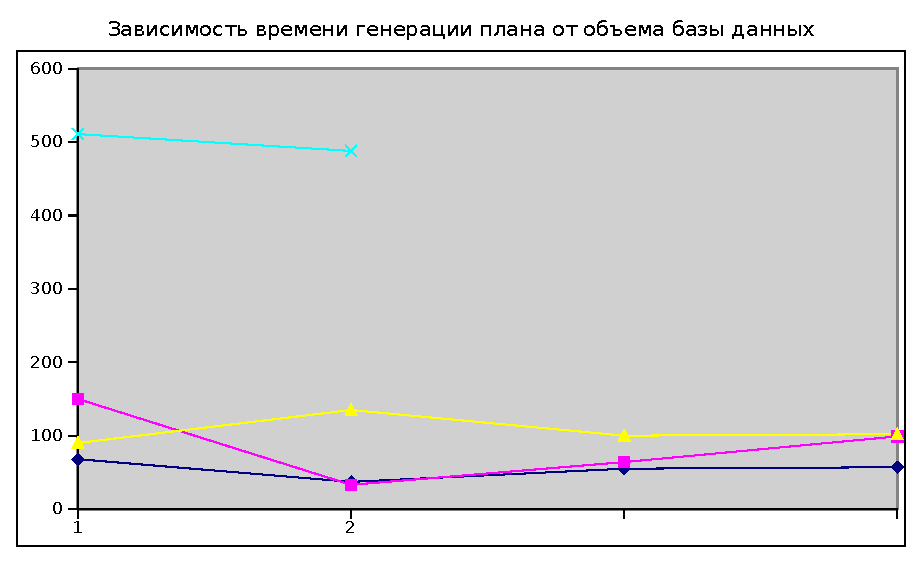
\includegraphics[width=0.8\linewidth]{plan_gen.eps}
	}
	\caption{Зависимость времени генерации плана от заполнения базы данных}
	\label{img::gen1}
\end{figure}

\begin{figure}[h]
	\noindent\centering{
		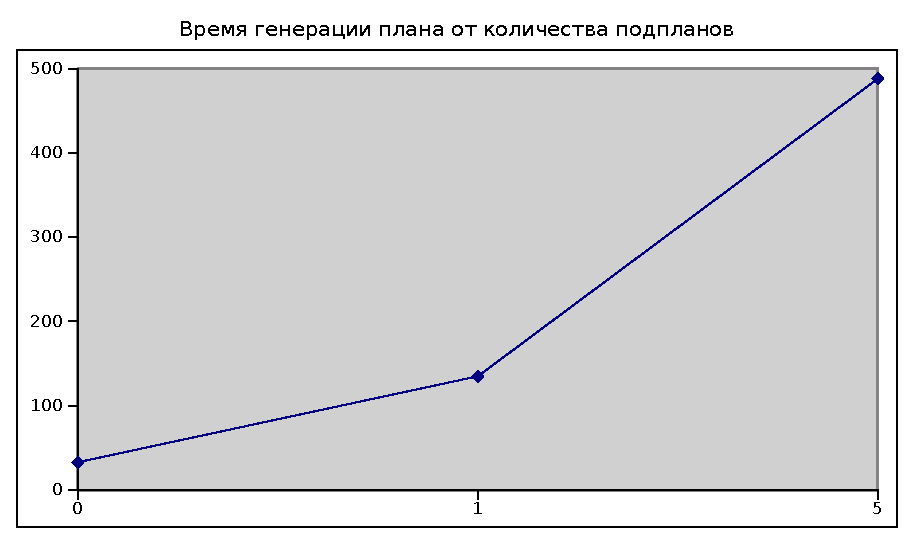
\includegraphics[width=0.8\linewidth]{plan_gen2.eps}
	}
	\caption{Зависимость времени генерации плана от количества подпланов}
	\label{img::gen2}
\end{figure}

На графиках (см \ref{img::gen1} и \ref{img::gen2}) можно видеть, что время генерации плана зависит от сложности 
запроса (количества вложенных запросов и сложности используемых операций). Если заполнение базы данных влияет на
время генерации плана, то по сравнению со сложностью запроса эта зависимость незначительна.

\begin{figure}[h]
	\noindent\centering{
		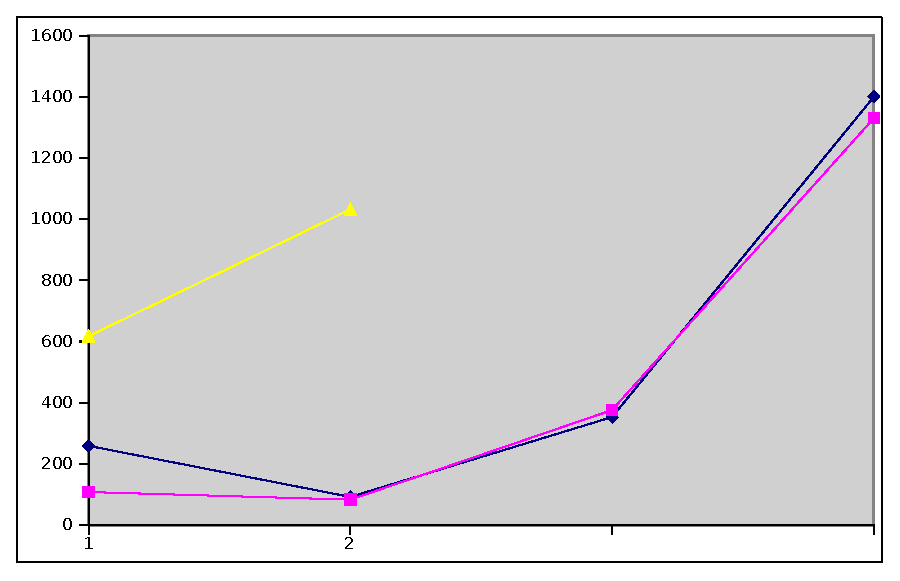
\includegraphics[width=0.8\linewidth]{plan_exec.eps}
	}
	\caption{Зависимость времени исполнения плана от заполнения базы данных (запросы 7.4, 8.1, 10.18)}
	\label{img::exec1}
\end{figure}

\begin{figure}[h]
	\noindent\centering{
		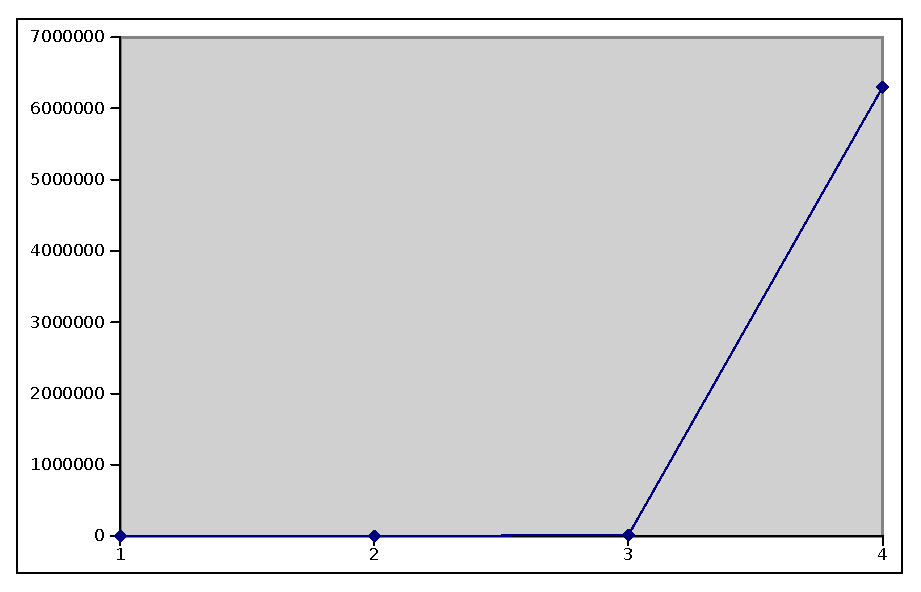
\includegraphics[width=0.8\linewidth]{plan_exec2.eps}
	}
	\caption{Зависимость времени исполнения плана от заполнения базы данных (запрос 15.9)}
	\label{img::exec2}
\end{figure}

Очевидно, что объем данных влияет на время исполнения запроса (см \ref{img::exec1} и \ref{img::exec2}), кроме того видно,
что сложность запроса так же влияет на время исполнения (по этой причине \ref{img::exec2} вынесен на отдельный график, так
как время его выполнения в несколько порядков больше).

Стоит отметить, что время выполнения запроса 15.9 на столько велико, что уже после исполнения скрипта $UpgradeSportDB3$
не получилось оценить время его выполнения в базе данных $JRS$.

Планы выполнения приведенных запросов используют следующие операции:
\begin{enumerate}
\item Filter (9 раз)

\item TableScan (9 раз)

\item Project (7 раз)

\item Sort (1 раз)

\item IndexOnlyFilter (1 раз)
\end{enumerate}

При изменении объемов базы данных план выполнения запросов оставался неизменным.

Теперь для сравнения преобразуем запрос 10.18 следующим образом:
\begin{lstlisting}
SELECT PlayerNo, Name
FROM Players, Matches
WHERE Players.PlayerNo=Matches.PlayerNo AND Matches.TeamNo = 1;
\end{lstlisting}

Результаты:
\begin{tabular}[t]{|c|c|c|c|c|}
\hline
Заполнение базы       &   1  &    2 &    3 &     4 \\
\hline
Время генерация плана &  95  &   58 &  103 &    62 \\
\hline
Время исполнения      & 132  &   90 &  142 &  1601 \\
\hline
\end{tabular}

Как видно время исполнения запроса в таком случае на порядок выше.

\paragraph{Вывод:}

Исходя из полученных данных можно сделать вывод, что время генерации плана выполнения может не зависеть
от объема базы данных, например в том случае, если конкретная база данных оценивая стоимость операций не учитывает размер
базы данных.

Кроме того как время выполнения так и время генерации плана завсит от структуры запроса, поэтому по возможности стоит избегать
вложенных запросов давая таким образом большую свободу оптимизатору запросов. Так как по сравнению с исполнением запроса, время
генерации плана в больших базах данных незначительно, то давая большую свободу оптимизатору вероятнее будет получена большая
производительность.
\end{document}
